\documentclass[12pt]{article}

\usepackage{blindtext} % Package to generate dummy text throughout this template 

% writing
\usepackage[utf8]{inputenc}
\usepackage{amsmath, amssymb, amsthm}
\usepackage{algorithm}
\usepackage[noend]{algpseudocode}
\linespread{1.5}
\usepackage[margin = 1in]{geometry}
\usepackage{microtype} % Slightly tweak font spacing for aesthetics
\usepackage[english]{babel} % Language hyphenation and typographical rules

% tikz
\usepackage{tikz}
\usepackage{pgfplots}
\usepackage{pgfplotstable}
\pgfplotsset{compat=1.13}

% fig
\usepackage{natbib, hyperref}
\usepackage{url}
\usepackage{graphicx}
\usepackage{float}
\usepackage{wrapfig}
\usepackage{multicol}

% misc
\usepackage{nomencl}
\usepackage[titletoc, page]{appendix}

% caption features
\usepackage{caption}
\usepackage{subcaption}
\usepackage{setspace}
\captionsetup{font={small, stretch=1.25}}
\let\Algorithm\algorithm
\renewcommand\algorithm[1][]{\Algorithm[#1]\setstretch{1.25}}

\hypersetup{
    colorlinks=true,
    linkcolor=black,      
    urlcolor=red,
    citecolor=green!75!black
}

\setlength{\parindent}{2em}
%\setlength{\parskip}{1.5em}
\graphicspath{ {images/} }

% nomenclature specs
\makenomenclature
\setlength{\nomitemsep}{-\parsep}
\renewcommand{\nomname}{List of Functions, Symbols \& Terms}
%% This code creates the groups
% -----------------------------------------
\usepackage{etoolbox}
\renewcommand{\nomgroup}[1]{%
    \item[\bfseries
    \ifstrequal{#1}{T}{Terms}{%
        \ifstrequal{#1}{S}{Symbols}{%
            \ifstrequal{#1}{F}{Functions}{}}%
    }]}
% -----------------------------------------

\newtheorem{mydef}{Definition}

\newcommand{\vect}[1]{\mathbf{#1}}  % vector
\newcommand{\matr}[1]{\mathbf{#1}}  % matrix
\newcommand{\tens}[1]{\mathbf{#1}}  % tensor
\newcommand{\mean}[1]{\overline{#1}}    % mean overline

\begin{document}
    % nomenclature
    \mbox{}
    % symbols
    \nomenclature[S]{$J$}{Number of locations in the dataset}
    \nomenclature[S]{$T$}{Number of time units for which data is available}
    \nomenclature[S]{$n_F$}{Number of features in the dataset $\matr{F}$ (length of $\matr{F}[v][u]$)}
    
    % functions
    \nomenclature[F]{softmax($\cdot$)}{Defined as softmax($z_i$) = $\frac{\exp(z_i)}{\sum_{i} \exp(z_i)}$}
    \nomenclature[F]{reLU($\cdot$)}{Defined as reLU($z$) = max(0, $z$)}
    \nomenclature[F]{batch-multiply($\cdot$)}{Operates on $m \times n \times p$ and $m \times p \times q$ tensors to give a $m \times n \times q$ tensor.}
    
    % terms
    \nomenclature[T]{Epoch}{One training/testing period; iteration}
    \nomenclature[T]{CPU ``set''}{\textit{All} operations done on the CPU}
    \nomenclature[T]{GPU ``set''}{\textit{Only Matrix/Tensor} operations done on the GPU, rest on the CPU}
    \nomenclature[T]{LP}{Linear Programming}
    \nomenclature[T]{LP Standard Format}{Arrangement of objective function and constraints operated on by library LP solvers - minimize [$\vect{c}^T \cdot \vect{x}$]; subject to [$\matr{A} \cdot \vect{x} \leq \vect{b}, \, x_i \geq 0$]}
    \nomenclature[T]{Tensor}{Multi-dimensional (usually more than 2 dimensions) array}
    \printnomenclature[1.5in]
    \cleardoublepage
    
    \tableofcontents
    \listoftables
    \listoffigures
    \cleardoublepage
    % main body
    \section{Introduction} \label{sec:Introduction}
    Optimizing predictive models on datasets that are obtained from citizen-science projects can be computationally expensive as these datasets grow in size with time. Consequently, models based on multiple-layered neural networks, Integer Programming and other optimization routines can prove increasingly difficult as the number of parameters increase, despite using the faster Central Processing Units (CPUs) in the market. Incidentally, it becomes difficult for citizen-science projects to scale if the organizers use CPUs to run optimization models. However, Graphical Processing Units (GPUs), which offer multiple cores to parallelize computation, can outperform CPUs in computing such predictive models if these models heavily rely on large-scale matrix multiplications. By using GPUs over CPUs to accelerate computation on a citizen-science project, the model could achieve better optimization in less time, enabling the project to scale.
    
    Part of the eBird project, which aims to ``maximize the utility and accessibility of the vast numbers of bird observations made each year by recreational and professional bird watchers'', Avicaching is a incentive-driven game trying to homogenize the spatial distribution of citizens' (agents') observations [cite website]. Since the dataset of agents' observations in eBird is geographically heterogeneous (concentrated in some places like cities and sparse in others), Avicaching homogenizes the observation set by rewarding agents who visit under-sampled locations \cite{Xue2016Avi1}. For the organizers, a more homogeneous observation dataset can enable \textit{better} mapping and generate more confidence in the dependent models' validity. 
    
    To accomplish this task of specifying rewards at different locations based on the historical records of observations, Avicaching would learn the change in agents' behavior when a certain sample of rewards were applied to the set of locations, and then distribute a newer set of rewards across the locations based on those learned parameters \cite{Xue2016Avi2}. This requirement naturally translates into a predictive optimization problem, which is implemented using multiple-layered neural networks and linear programming.
    
    \subsection{Important Questions}
    Although the previously devised solutions to Avicaching were conceptually effective \cite{Xue2016Avi1}\cite{Xue2016Avi2}, using CPUs to solve Mixed Integer Programming and shallow neural networks made them impractical to scale. While wider applicability would have increased homogeneity in the observation set, Mixed Integer Programming formulations made it hard for Avicaching to scale and influence a larger segment of eBird. Solving the problems faster would have also allowed organizers to find better results (more optimized). These concerns, which form the pivot for our research, are concisely described in next sections.
    
    \subsubsection{Solving Faster} \label{sec:Important Questions - Solving Faster}
    We were interested in using GPUs to run our models, with their growing capability to accelerate problems in Artificial Intelligence and Machine Learning - more specifically, large matrix and tensor operations. Newer generation NVIDIA GPUs equipped with thousands of CUDA (NVIDIA's parallel computing API) cores can empower Avicaching's organizers to scale the game, if it is based on extensive simple arithmetic operations on tensors and matrices, rather than logical steps (why? - reasoned in Section \ref{sec:Computation Using GPUs}). Since even the faster CPUs (in the range of Intel Core i7 chipsets and faster) are sequential in processing and do not provide as comparable parallel processing as GPUs do, we can solve the problem much faster. \textbf{But how much faster?}
    
    \subsubsection{Better Results} \label{sec:Important Questions - Better Results}
    The previous model for learning the parameters in agents' change of behavior on a fixed set of rewards delivered predictions that differed 26\% from Ground Truth \cite[// todo]{Xue2016Avi2}, which was used to distribute a new set of rewards on a budget. If we could get closer to the Ground Truth, i.e., learn the parameters for the change better, we could distribute a new set of rewards based on better learning and prediction. Since the organizers need the \textit{best} distribution of rewards (key aspect in testing the model), we would need a set of learned parameters that give lesser difference from the Ground Truth (in terms of Normalized Mean Squared Error \cite[// todo]{Xue2016Avi2}). In a gist, \textbf{can we learn the parameters better}, and \textbf{what is the best allocation of rewards?}
    
    \subsubsection{Adjusting the Model's Features} \label{sec:Important Questions - Adjusting the Model's Features}
    Once our model starts delivering better results than the previously devised models, one thinks if one can change some characteristics of the model (known as hyper-parameters such as learning rate) to get even better results (though one could also build a better model too). While a goal of ``getting better results'' may seem like an unending strife (any one can never get satisfied), there is a trade-off with practicality as these adjustments take time and computation power to test - and we don't have unlimited resources. Therefore, we ask if one could \textbf{reasonably adjust hyper-parameters to improve performance and optimization.} By ``reasonable adjustments'' we mean changes that improve performance by more than 5 times using comparable resources.
    
    \subsection{Computation Using GPUs} \label{sec:Computation Using GPUs}
    // todo
    
    \blindtext
    
    \section{Problem Formulation} \label{sec:Problem Formulation}
    Since NVIDIA General Purpose GPUs enable faster computation on tensors and matrices, accelerated through CUDA and cuDNN, both the Identification (Section \ref{sec:Identification Problem}) and the Pricing Problem (Section \ref{sec:Pricing Problem}) were formulated as tensor-based 3-layered and 2-layered neural networks respectively using the PyTorch library.
    
    \subsection{Identification Problem} \label{sec:Identification Problem}
    As discussed in Section \ref{sec:Introduction}, the model should learn parameters that caused the change in agents' behavior when a certain set of rewards was applied to locations in the experiment region. Learning those parameters will help us understand how agents behave with a fixed reward distribution, and will enable organizers to redistribute rewards based on that behavior.
    
    Specifically, given datasets $\vect{y_t}$ and $\vect{x_t}$ of agents' visit densities, with and without the rewards $\vect{r_t}$, we want to find weights $\matr{w_1}$ and $\matr{w_2}$ that caused the change from $\vect{x_t}$ to $\vect{y_t}$, factoring in possible influence from environmental factors $\matr{f}$ and distances between locations $\matr{D}$. Although the original model proposed to learn a single set of weights $\matr{w}$ \cite{Xue2016Avi2}, this proposed model considers two sets of weights $\matr{w_1}$ and $\matr{w_2}$ as it may theoretically result into higher accuracy and lower loss. Mathematically, the model can be formulated as:
    \begin{equation} \label{eq:iden_problem}
        \begin{aligned}
            & \underset{\matr{w_1}, \matr{w_2}}{\text{minimize}}
            & & Z_I(\matr{w_1}, \matr{w_2}) = \sum_{t} (\omega_t(\vect{y_t} - \matr{P}(\matr{f}, \vect{r_t}; \matr{w_1}, \matr{w_2})\vect{x_t}))^{2}
        \end{aligned}
    \end{equation}
    where $\omega_t$ is a set of weights (not a learnable parameter) at time $t$ capturing penalties relative to how strongly we want to homogenize locations at time $t$. In other words, it highlights if the organizer wishes higher homogeneity at one time over another. Elements $p_{u, v}$ of $\matr{P}$ are given as:
    \begin{equation} \label{eq:puv_equation}
    p_{u, v} = \frac{\exp(\matr{w_2} \cdot \text{reLU} (\matr{w_1} \cdot [d_{u, v}, \vect{f_{u}}, r_{u}]))}{\sum_{u'} \exp(\matr{w_2} \cdot \text{reLU} (\matr{w_1} \cdot [d_{u', v}, \vect{f_{u'}}, r_{u'}]))} = \frac{\exp(\Gamma_{u, v})}{\sum_{u'}\exp(\Gamma_{u', v})} = \text{softmax}(\Gamma_{u, v})
    \end{equation}
    To optimize the loss value $Z_I(\matr{w_1}, \matr{w_2})$ (Equation \ref{eq:iden_problem}), the neural network learns the set of weights through multiple epochs of backpropagating the loss using gradient descent. Furthermore, the program processes the dataset before feeding to the network to avoid unnecessary sub-epoch iterations and to promote batch operations on tensors. 
    
    \subsubsection{Structure of Input Dataset for Identifying Weights} \label{sec:Structure of Input Dataset for Identifying Weights}
    \begin{figure}[H]
        \begin{subfigure}{.64\textwidth}
            \centering
            \includegraphics[width=\linewidth]{weights_input_dataset}
            \caption{A Tensor representing the Input Dataset $\matr{F}$}
            \label{fig:A Tensor representing the complete Input Dataset}
        \end{subfigure}
        \begin{subfigure}{.35\textwidth}
            \centering
            \includegraphics[width=\linewidth]{zoomup_Fuv}
            \caption{Contents of $\matr{F}[v][u]$}
            \label{fig:Zoomed-in contents of Fvu}
        \end{subfigure}
        \caption{Visual representation of the Input Dataset}
        \label{fig:Visual representation of the Input Dataset}
    \end{figure}
    Since preprocessing the dataset impacts the efficiency of the network, the input dataset, comprising of distance between locations $\matr{D}$, environmental features $\vect{f}$ and given rewards $\vect{r_t}$ (all normalized), is built in a specific manner. Since GPUs are efficient in operating on matrices and tensors, the input dataset is built into a tensor (Figure \ref{fig:A Tensor representing the complete Input Dataset}) such that batch operations could be performed on slices $\matr{F}[v]$.
    
    Another advantage of building the dataset as a tensor comes with the PyTorch library, which provides convenient handling and transfer of tensors residing on CPUs and GPUs. Algorithm \ref{alg:Constructing the Input Dataset} describes the steps to construct this dataset.
    
    \begin{algorithm}
        \caption{Constructing the Input Dataset} \label{alg:Constructing the Input Dataset}
        \begin{algorithmic}[1]
            \Function{Build-Dataset}{$\matr{D}, \matr{f}, \matr{r_t}$}
            \State $\matr{D} \gets \Call{Normalize}{\matr{D}}$\Comment{$\matr{D}[u][v]$ is the distance between locations $u$ and $v$}
            \State $\vect{f} \gets \Call{Normalize}{\mathbf{f}, axis = 0}$\Comment{$\mathbf{f}[u]$ is a vector of env. features at location $u$}
            \State $\vect{r_t} \gets \Call{Normalize}{\vect{r_t}, axis = 0}$\Comment{$\vect{r_t}[u]$ is the reward at location $u$}
            \For{$v = 1, 2, \dots, J$}
                \For{$u = 1, 2, \dots, J$}
                    \State $\tens{F}[v][u] \gets [\matr{D}[v][u], \vect{f}[u], \vect{r_t}[u]]$ \Comment{As depicted in Figure \ref{fig:Zoomed-in contents of Fvu}}
                 \EndFor
            \EndFor
            \State \Return $\matr{F}$
            \EndFunction
        \end{algorithmic}
    \end{algorithm}

    \subsubsection{Minimizing Loss for the Identification Problem} \label{sec:Minimizing Loss for the Identification Problem}
    As shown in Figure \ref{fig:Neural network designed for the Identification Problem}, the neural network is made of 3 fully connected layers - the input layer, the hidden layer with rectified Linear Units (reLU), and the output layer generating the results using the softmax$(\cdot)$ function. The network can also be visualized as a collection of 1-dimensional layers (Figure \ref{fig:Side view of the network}), with the softmax$(\cdot)$ calculated on the collection's output.
    \begin{figure}[!htbp]
        \begin{subfigure}{.64\textwidth}
        \includegraphics[width=\textwidth]{weights_net}
        \caption{3-dimensional view of the network slice, taking in $\matr{F}[v]$}
        \label{fig:3-dimensional view of the network slice, taking in Fv}
        \end{subfigure}
        \begin{subfigure}{.35\textwidth}
            \includegraphics[width=\textwidth]{weights_net_side}
            \caption{Side view of the network}
            \label{fig:Side view of the network}
        \end{subfigure}
        \caption{Neural network designed for the Identification Problem}
        \label{fig:Neural network designed for the Identification Problem}
    \end{figure}
    It is important to clarify that the network in Figure \ref{fig:3-dimensional view of the network slice, taking in Fv}, which takes in $\matr{F}[v]$ as shown, is a slice of the original network, which takes in the complete tensor $\matr{F}$ and computes the complete result $\matr{P}^{T}$  per iteration of $t$. In other words, the input and the hidden layers are 3-dimensional, and the output layer is 2-dimensional. Since it is difficult to visualize the complete network on paper, slices of the network are depicted in Figure \ref{fig:3-dimensional view of the network slice, taking in Fv}. Algorithm \ref{alg:Algorithm for the Identification Problem} details the steps for learning the parameters $\matr{w_1}$ and $\matr{w_2}$ based on Equations \ref{eq:iden_problem} \& \ref{eq:puv_equation}.
    
    \begin{algorithm}
        \caption{Algorithm for the Identification Problem} \label{alg:Algorithm for the Identification Problem}
        \begin{algorithmic}[1]
            \State $\matr{w_1} \gets \Call{Random}{\;(J,n_F,n_F)\;}$\Comment{$\matr{w_1}$ has dimensions $J \times n_F \times n_F$}
            \State $\matr{w_2} \gets \Call{Random}{\;(J,n_F,1)\;}$\Comment{$\matr{w_2}$ has dimensions $J \times n_F \times 1$}
            \For{$e = 1, 2, \dots, \text{Epochs}$}
                \State $loss \gets 0$
                \For{$t = 1, 2, \dots, T$}
                    \State $\matr{F} \gets \Call{Build-Dataset}{\matr{D}, \matr{f}, \matr{r}[t]}$\Comment{Defined in Algorithm \ref{alg:Constructing the Input Dataset}}
                    \State $\matr{H} \gets  \text{reLU}(\Call{Batch-Multiply}{\matr{F}, \matr{w_1}})$
                    \State $\matr{O} \gets \text{softmax}(\Call{Batch-Multiply}{\matr{H}, \matr{w_2}})$
                    \State $\matr{P} \gets \matr{O}^T$
                    \State $loss \gets loss + (\omega(\matr{y}[t] - \matr{P} \cdot \matr{x}[t]))^2$
                \EndFor
                \State $\Call{Gradient-Descent}{loss, \matr{w_1}, \matr{w_2}}$
                \State $\matr{w_1}, \matr{w_2} \gets \Call{Update-Using-Gradients}{\matr{w_1}, \matr{w_2}}$
                \State $\Call{Log-Info}{e, loss}$
            \EndFor
        \end{algorithmic}
    \end{algorithm}
    
    \subsection{Pricing Problem} \label{sec:Pricing Problem}
    After learning the set of weights $\matr{w_1}$ and $\matr{w_2}$ highlighting the change in agents' behavior to collect observations, the Pricing Problem aims to redistribute rewards to the all locations such that the predicted behavior of agents influenced by the new set of rewards is homogeneous. Thus, given a budget of rewards $\mathcal{R}$, this optimization problem can be expressed as:
    \begin{equation} \label{eq:pricing_problem}
        \begin{aligned}
            & \underset{\vect{r}}{\text{minimize}}
            & & Z_P(\vect{r}) = \frac{1}{n}\lVert \vect{y} - \mean{\vect{y}} \rVert\\
            & \text{subject to}
            & & \vect{y} = \matr{P}(\matr{f}, \vect{r}; \matr{w_1}, \matr{w_2}) \, \vect{x}\\
            &&& \sum_{i} r_i \leq \mathcal{R}\\
            &&& r_i \geq 0
        \end{aligned}
    \end{equation}
    where elements of $\matr{P}$ are defined as in Equation \ref{eq:puv_equation}.
    
    To allocate the rewards $\vect{r}$ optimally, the calculations for the pricing problem are akin to that for the Identification Problem (Section \ref{sec:Identification Problem}). However, since only 1 set of rewards need to be optimized, we use an altered 2-layer network instead of the 3-layer network used to identify the weights. While Equation \ref{eq:pricing_problem} looks like a typical Linear Programming (LP) problem, only a part of the formulation uses LP to constrain the rewards. Calculation for $\matr{P}$ is modeled as a 2-layer network that minimizes the loss function $Z_P(\vect{r})$ using gradient descent. Although this use of a neural network may seem similar to that of the Identification Problem, there are major changes in the structure of the network used here. These alterations for the Pricing Problem and differences from the Identification Problem are discussed further in the following sections. Specific Implementation details, with code optimizations and more data preprocessing, are described in Appendix \ref{sec:Implementation}.
    
    \subsubsection{Input Dataset for Finding Rewards}
    Since it is the set of rewards $\vect{r}$ that need to be optimized, they must serve as the ``weights'' of the network (note that ``weights'' here refer to the edges of this network and not to the set of calculated weights $\matr{w_1}$ and $\matr{w_2}$). Therefore, the rewards $\vect{r}$ are no longer fed into the network but are its characteristic. Instead, the calculated weights $\matr{w_1}$ are fed into the network, and are ``weighted'' by the rewards.
    
    The observation density datasets, $\matr{x}$ and $\matr{y}$, are also aggregated for all agents such that they give information in terms of locations $u$ only. This is also why rewards $\vect{r}$ does not depend on $t$ - we want a generalized set of rewards for all time $t$ per location $u$. Therefore, the algorithm for constructing $\matr{F}$ (Section \ref{sec:Structure of Input Dataset for Identifying Weights}) is same as Algorithm \ref{alg:Constructing the Input Dataset} but with a change - $\vect{r_t}$ replaced by $\vect{r}$.
    
    \subsubsection{Optimizing \& Constraining Rewards} \label{sec:Optimizing and Constraining Rewards}
    The algorithm for finding $\matr{P}$ is very similar to Phase 1 of Algorithm \ref{alg:Algorithm for the Identification Problem} but without any epochs of $t$, as $\vect{x}, \vect{y}, \vect{r}$ are vectors rather than matrices. Also, since the program (Algorithm \ref{alg:Solving the Pricing Problem}) would predict $\vect{y}$, it does not need labels $\vect{y}$ as a dataset. Although Algorithm \ref{alg:Solving the Pricing Problem} might look arcane in the logic flow, it is straightforward - as displayed in Figure \ref{fig:Logic Flow of Algorithm Pricing Problem}. The algorithm only arranges the commands in a particular way to optimize implementation and execution.
    \begin{figure}[!htbp]
        \centering
        \includegraphics[width=\textwidth]{logic_alg_pricing}
        \caption{Logic Flow of Algorithm \ref{alg:Solving the Pricing Problem}}
        \label{fig:Logic Flow of Algorithm Pricing Problem}
    \end{figure}
    \begin{algorithm}
        \caption{Solving the Pricing Problem} \label{alg:Solving the Pricing Problem}
        \begin{algorithmic}[1]
            \Function{Forward}{$\matr{D}, \matr{f}, \vect{r}, \matr{w_1}, \matr{w_2}, \vect{x}$}
            \State $\matr{F} \gets \Call{Build-Dataset}{\matr{D}, \matr{f}, \vect{r}}$\Comment{Defined in Algorithm \ref{alg:Constructing the Input Dataset}}
            \State $\matr{O}_1 \gets \text{reLU}(\Call{Batch-Multiply}{\matr{F}, \matr{w_1}})$
            \State $\matr{O}_2 \gets \text{softmax}(\Call{Batch-Multiply}{\matr{O}_1, \matr{w_2}})$
            \State $\matr{P} \gets \matr{O}_2^T$
            \State $\vect{y} \gets \matr{P} \cdot \vect{x}$
            \State \Return $\lVert \vect{y} - \mean{\vect{y}} \rVert / J$
            \EndFunction
            \vspace*{-.7\baselineskip}\Statex\hspace*{\dimexpr-\algorithmicindent-2pt\relax}\rule{\textwidth}{0.1pt}%
            \Statex\hspace*{-\algorithmicindent}\textbf{Main Script}%
            \vspace*{-.5\baselineskip}\Statex\hspace*{\dimexpr-\algorithmicindent-2pt\relax}\rule{\textwidth}{0.1pt}% horizontal rule
            \State $\vect{r} \gets \Call{Random}{\;(J)\;}$\Comment{$\vect{r}$ has dimensions $J$}
            \State $loss \gets \Call{Forward}{\matr{D}, \matr{f}, \vect{r}, \matr{w_1}, \matr{w_2}, \vect{x}}$
            \For{$e = 1, 2, \dots, \text{Epochs}$}
                
            \State $\Call{Gradient-Descent}{loss, \vect{r}}$
            \State $\vect{r} \gets \Call{Update-Using-Gradients}{\vect{r}}$
            \State $\vect{r} \gets \Call{LP}{\vect{r}, \mathcal{R}}$\Comment{LP($\cdot$) explained in Section \ref{sec:Optimizing and Constraining Rewards}}
            \State $loss \gets \Call{Forward}{\matr{D}, \matr{f}, \vect{r}, \matr{w_1}, \matr{w_2}, \vect{x}}$
            \State $\Call{Log-Best-Rewards}{loss, \vect{r}}$\Comment{Records $\vect{r}$ with the lowest $loss$ yet}
            \EndFor
        \end{algorithmic}
    \end{algorithm}

    After updating the rewards, the program constrains them using LP($\cdot$) such that $\sum_{i}r_i \leq \mathcal{R}$ and $r_i \geq 0$. To do so, the LP($\cdot$) finds another set of rewards $\vect{r'}$ such that the absolute difference between new and old rewards ($\sum_{i}|r'_i - r_i|$) is minimum. The mathematical formulation is given in Equation \ref{eq:lp_math_constrain_rewards}, which was implemented (see Appendix \ref{sec:Implementation}) using SciPy's Optimize Module \cite{SCPOptimizeDocs}. Since the module supports a standard format for doing linear programming, Equation \ref{eq:lp_code_constrain_rewards} (after rearranging constraints and building $\matr{A}, \vect{b}$ and $\vect{c}$) is used, which is mathematically equivalent to Equation \ref{eq:lp_math_constrain_rewards}.
    \begin{multicols}{2}
        \begin{equation} \label{eq:lp_math_constrain_rewards}
            \begin{aligned}\\
                & \underset{\vect{r'}}{\text{minimize}}
                & & \sum_{i}|r'_i - r_i|\\
                & \text{subject to}
                & & \sum_{i}r'_i \leq \mathcal{R}\\
                &&& r_i \geq 0\\ \\
            \end{aligned}
        \end{equation}\break
        \begin{equation} \label{eq:lp_code_constrain_rewards}
            \begin{aligned}
                & \underset{[\vect{r'}, \vect{u}]}{\text{minimize}}
                & & \sum_{i} u_i\\
                & \text{subject to}
                & & r'_i - r_i \leq u_i\\
                &&& r_i - r'_i \leq u_i\\
                &&& \sum_{i} r'_i \leq \mathcal{R}\\
                &&& r'_i, u_i \geq 0
            \end{aligned}
        \end{equation}
    \end{multicols}
    
    \section{Experiment Specifications} \label{sec:Experiment Specifications}
    \begin{mydef} \label{def:GPU Speedup}
        GPU Speedup: Ratio of increase in time elapsed in GPU and that of CPU per unit increase in batch-size.
    \end{mydef}
    To test both our models, we conducted several tests for optimization and GPU speedup over CPU. After initializing all parameters randomly and reading data from files, the models were run for 1000 to 10000 epochs depending on the complexity of the model and any potential benefits emerging with more epochs.
    
    A Dell Precision Tower 3620 with Intel Core i7-7700K Processor [], 16GB RAM and NVIDIA Quadro P4000 GPU [] was used for all experiments. These experiments were either optimization tests on original datasets or GPU speedup tests randomly generated datasets. We believe that speedup tests on original datasets would give similar results, though we used randomly generated datasets because it was easier to scale and build random datasets of different batch-sizes.
    
    Note that operations in the scripts were \textit{distributed between} CPU and GPU when GPU is mentioned as ``set'', while the operations were executed \textit{only} on the CPU when the ``CPU'' is mentioned as set. Since GPUs are inferior than CPUs at handling most operations other than simple arithmetic matrix ones, we used - and recommend using - both the CPU and the GPU in the former case (GPU ``set'') to handle operations each is superior at. However, since the models in Sections \ref{sec:Identification Problem} and \ref{sec:Pricing Problem} (not the full scripts) are primarily arithmetic operations on matrices and tensors, it is clear that they were executed on the GPU when it was ``set'' and on the CPU when the CPU was ``set''.
    
    On the algorithm side, we used Adam's algorithm for \textsc{Gradient-Descent}($\cdot$), after testing performances of several algorithms including but not limited to Stochastic Gradient Descent (SGD) \cite{SGD}, Adam's Algorithm \cite{Adam} and Adagrad \cite{Adagrad} (PyTorch lets you choose the corresponding function). Since Adam's algorithm was found to work best with both models over all test runs, all experiments were done using Adam's algorithm. Hence, all results were also obtained using Adam's algorithm.
    
    \subsection{Running the Identification Problem's Model} \label{sec:Running the Identification Problem's Model}
    \subsubsection{Optimizing the Original Dataset} \label{sec:Identification Problem-Optimizing the Original Dataset}
    The 3-layered neural network was run for 10000 epochs on the original dataset, which was split 80:20 for training and testing sets, with different learning rates = $\{10^{-2}, 10^{-3}, 10^{-4}, 10^{-5}\}$. Since we were aiming for optimization, we ran multiple tests (5 different seeds with each learning rate) of the model only with the GPU ``set''.
    
    To compare this model's optimization results with other model structures, the previously studied 2-layered network \cite{Xue2016Avi2} and a 4-layered neural network were used. The 4-layered network had another hidden layer with reLU, equivalent to the hidden layer in the current 3-layered network (Figure \ref{fig:3-dimensional view of the network slice, taking in Fv}). The results from the 2-layered network were obtained from the previous study, and those from the 4-layered network were attained on the same original dataset with same parameter values (learning rates, epochs etc.).
    
    \subsubsection{Testing GPU Speedup on the Random Dataset} \label{sec:Identification Problem-Testing GPU Speedup on the Random Dataset}
    After generating random datasets of different sizes ($T = 17, 85, 173$ - Section \ref{sec:Minimizing Loss for the Identification Problem}, we ran our 3-layered model on each dataset size with different seeds with both GPU and CPU ``set'', logging time elapsed. The total time elapsed was averaged for a batch-size on a device, which were used to generate scatter/line plots (Section \ref{sec:IdProbRes - GPU}).
    
    \subsection{Running the Pricing Problem's Model} \label{sec:Running the Pricing Problem's Model}
    \subsubsection{Optimizing the Original Dataset} \label{sec:Pricing Problem-Optimizing the Original Dataset}
    After obtaining the set of weights $\matr{w_1}$ and $\matr{w_2}$ optimized using different seeds, we tested to find the best rewards (with the lowest loss - Equation \ref{eq:pricing_problem}) with random $\vect{r}$ initiation. To obtain the best rewards, the model was run on all sets of weights obtained from the Identification Problem for 1000 epochs with different learning rates.
    
    Two sets of rewards were tested for loss values as baseline comparisons to our model - a randomly generated set, and another with elements proportional to the reciprocal of number of visits at each location. While the former was a random baseline, the latter captured the idea of allocating higher rewards to relatively under-sampled locations. The average loss values (on different sets of weights) were compared for all tests with the baselines.
    
    \subsubsection{Testing GPU Speedup on the Random Dataset} \label{sec:Pricing Problem-Testing GPU Speedup on the Random Dataset}
    After generating random datasets of different sizes ($J = 11, 55, 116$ - Section \ref{sec:Minimizing Loss for the Identification Problem}), we ran our 3-layered model on each dataset size with different seeds with both GPU and CPU ``set''.
    
    Since PyTorch does not provide a GPU-accelerated Simplex LP solver, we relied on SciPy's Optimize Module to solve the that part of the model. Since SciPy's implementation does not utilize the GPU \textit{conspicuously}, we expected the LP problem to be executed on the CPU and thus deliver equal runtimes in both GPU and CPU ``set'' configurations.
    
    \section{Results} \label{sec:Results}
    \subsection{Identification Problem's Results} \label{sec:Identification Problem's Results}
    \subsubsection{Optimization Results} \label{sec:IdProbRes - Optimization}
    Minimizing the loss function in the Identification Problem (Section \ref{sec:Identification Problem}) on the original dataset for 10000 epochs took an average of 1260.62 seconds with the GPU ``set''.
    \begin{itemize}
        \item The average loss values at the end of 10000 epochs were 0.04 on the training set and 0.14 on the test set.
        \item The average loss values for the 4-layered model (for comparison) with same experiment specifications were 0.14 on the training set and 0.49 on the test set.
    \end{itemize}
    \begin{figure}[!htbp]
        \centering
        \begin{minipage}{.49\textwidth}
            \centering
            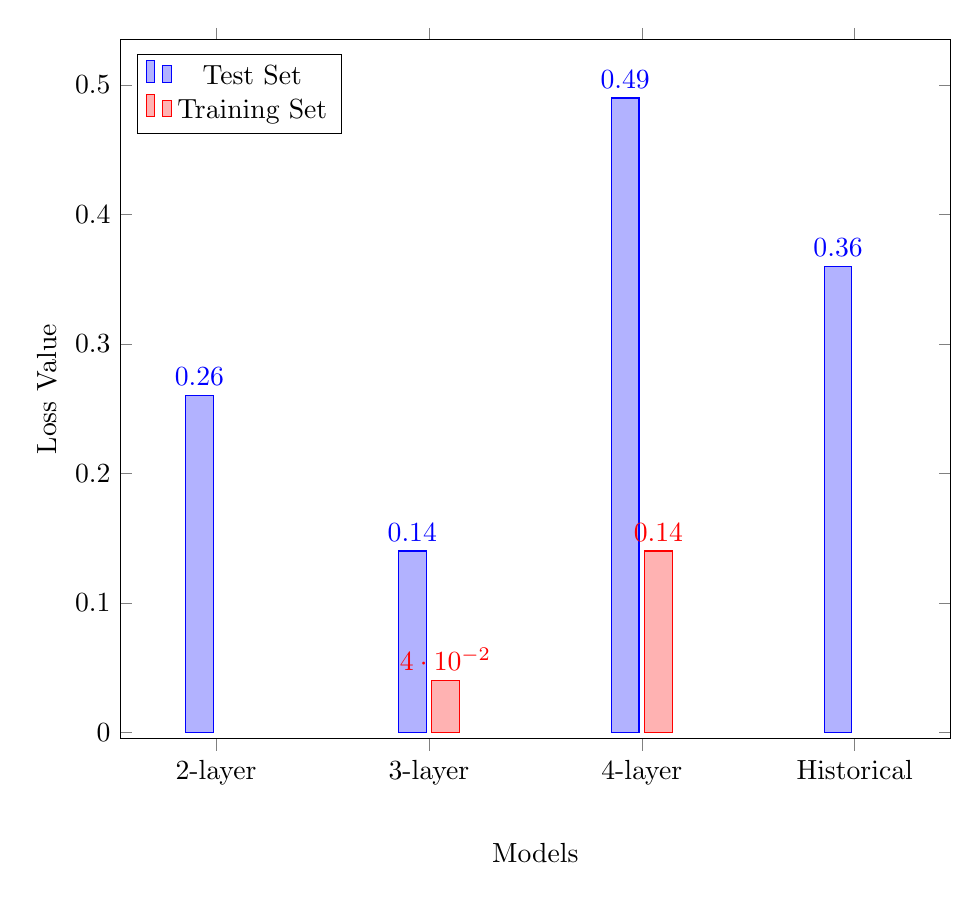
\begin{tikzpicture}
                \begin{axis}[
                    ybar,
                    width=\textwidth,
                    enlarge x limits=0.15,
                    legend style={at={(0.02,0.98)},
                        anchor=north west,legend columns=1},
                    ylabel={Loss Value},
                    symbolic x coords={2-layer,3-layer,4-layer, Historical},
                    xtick=data,
                    nodes near coords,
                    nodes near coords align={vertical},
                    xlabel={Models},
                    xlabel style={yshift=-.5cm}
                ]
                \addplot coordinates {(2-layer,0.26) (3-layer,0.14) (4-layer,0.49) (Historical, 0.36)};
                \addplot coordinates {(3-layer,0.04) (4-layer,0.14)};
                \legend{Test Set,Training Set}
                \end{axis}
            \end{tikzpicture}
            \caption[Comparison of Loss Values from Different Models of the Identification Problem]{Comparison of Loss Values from Different Models of the Identification Problem: Loss values for the training set are inevitably lower than that for the test set, which should be the basis for comparison}
            \label{fig:Comparison of Loss Values from Different Models of the Identification Problem}
        \end{minipage}\hfill
        \begin{minipage}{.49\textwidth}
            \centering
            \includegraphics[width=\textwidth]{weights_map_plot_3}
            \caption[Predicted Probabilities of Agents Visiting Each Location Plotted on a Map (Latitude, Longitude) Representing Tompkins and Cortland Counties, NY]{Predicted Probabilities of Agents Visiting Each Location Plotted on a Map (Latitude, Longitude) Representing Tompkins and Cortland Counties, NY: Dark dots represent high prediction of visits. This can be compared to the plots for the 2-layered network and other models \cite[Figure 3]{Xue2016Avi2}.}
            \label{fig:Predicted Probabilities of Agents Visiting Each Location Plotted on a Map}
        \end{minipage}
    \end{figure}
    As depicted in Figure \ref{fig:Comparison of Loss Values from Different Models of the Identification Problem}, our 3-layered neural network outperformed the previous 2-layered model by 0.12 units (12\% more closer to Ground Truth - $\matr{y}$) \cite[Table 1]{Xue2016Avi2}, and also produced much better results (35\% more closer to Ground Truth) than the 4-layered model.
    
    We also generated the predicted probabilities of the agents visiting each location ($\matr{P} \cdot \matr{x}$) in the Test Set, and plotted it onto a map marked by the locations' latitudes and longitudes. Figure \ref{fig:Predicted Probabilities of Agents Visiting Each Location Plotted on a Map} shows such a plot generated by the 3-layered network, where each dot represents a location.
    
    Although there remained a 10\% difference (0.10 loss units) in the values of training and testing set, the 3-layered model was not starkly overfitting as an average \textit{end} difference of $10.7\pm5.5\%$ persisted for many epochs, instead of increasing and tuning more to the training set. On the other hand, overfitting is more remarked in the case of 4-layered model, producing an average \textit{end} difference of $34.8\pm8.9\%$, but erratically hovering between 20\% and 50\%. This result is shown in Figure \ref{fig:Train & Test Loss Values' Plots of Different Models} with plots of loss values at each epoch for the 3- and the 4-layered network.
    \begin{figure}[!htbp]
        \centering
        \begin{subfigure}{.49\textwidth}
            \centering
            \includegraphics[width=\textwidth]{weights_train_test_loss_3_plot}
            \caption{Plot for 3-layered Model}
            \label{fig:Plot for 3-layered Model}
        \end{subfigure}
        \begin{subfigure}{.49\textwidth}
            \centering
            \includegraphics[width=\textwidth]{weights_train_test_loss_4_plot}
            \caption{Plot for 4-layered Model}
            \label{fig:Plot for 4-layered Model}
        \end{subfigure}
        \caption[Train \& Test Loss Values' Plots for One of the Runs of Different Models]{Train \& Test Loss Values' Plots for One of the Runs of Different Models: Both networks learn the set of weights quickly, as displayed in the steep descent in loss values before $\approx$ 1000 epochs. This quick learning is due to the choice of \textsc{Gradient-Descent}($\cdot$) function - Adam's algorithm \cite{Adam}. Other algorithms like SGD \cite{SGD} and Adagrad \cite{Adagrad} learn relatively slowly.}
        \label{fig:Train & Test Loss Values' Plots of Different Models}
    \end{figure}

    \subsubsection{GPU Speedup Results} \label{sec:IdProbRes - GPU}
    Running on batches of sizes $T = 17, 85, 173$ on a randomly generated dataset, with both GPU and CPU ``set'' separately, we obtained full  execution time (including both training and testing) information. The average results (3 different seeds for each batch) are plotted in Figure \ref{fig:Execution Times of Different Batch-Sizes with GPU and CPU ``set'' Separately}, which show promising GPU speedup over CPU figures for any batch size - for every unit increase in batch-size $T$, CPU ``set'' takes $\approx$ 4.66 seconds, while GPU ``set'' takes only $\approx$ 0.74 more seconds (slopes of best-fit trendlines).
    \begin{figure}[!htbp]
        \centering
        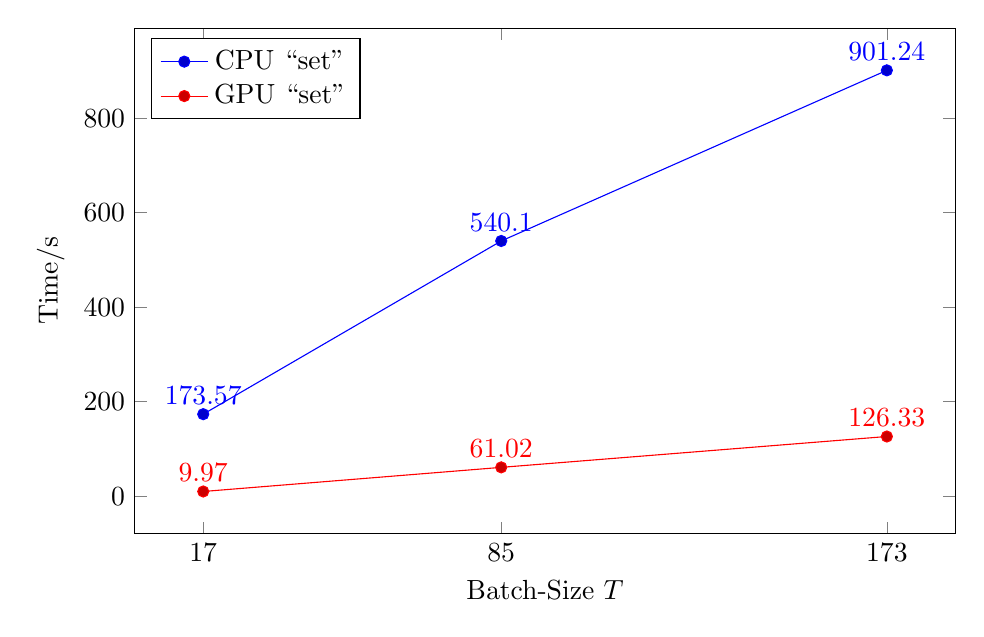
\begin{tikzpicture}
            \begin{axis}[
                width=12cm,
                height=8cm,
                xtick=data,
                xlabel={Batch-Size $T$},
                ylabel={Time/s},
                y tick label style={/pgf/number format/1000 sep=},
                extra y tick style={grid=major, tick label style={xshift=-1cm}},
                legend style={at={(0.02,.98)},
                    anchor=north west},
                nodes near coords,
            ]
            \addplot+ [mark=*,] coordinates {(17,173.57) (85,540.10) (173,901.24)};  % cpu
            \addplot+ [mark=*,] coordinates {(17,9.97) (85,61.02) (173,126.33)};  % gpu
            \legend{CPU ``set'',GPU ``set''}
            \end{axis}
        \end{tikzpicture}
        \caption[Finding Weights - Execution Times of Different Batch-Sizes $T$ with GPU and CPU ``set'' Separately]{Finding Weights - Execution Times of Different Batch-Sizes $T$ with GPU and CPU ``set'' Separately: Scaling on a GPU is more efficient (about $\frac{4.66}{0.74} \approx 6.25$ times) than doing so on a CPU.}
        \label{fig:Execution Times of Different Batch-Sizes with GPU and CPU ``set'' Separately}
    \end{figure}

    \subsection{Pricing Problem's Results} \label{sec:Pricing Problem's Results}
    \subsubsection{Optimization Results} \label{sec:PriProbRes - Optimization}
    After doing tests on the original for loss minimization and comparing with the baseline scores, we found that our model was performing $\approx$ 8 times better than both randomly generated and proportionally distributed rewards. Table \ref{tab:Loss Values Calculated from Different Sets of Rewards} lists the average loss values obtained on each type of reward allocation (model's predicted, random and proportionate).
    \begin{table}[!htbp]
        \centering
        \caption[Loss Values Calculated from Different Sets of Rewards]{Loss Values Calculated from Different Sets of Rewards: The values are small because the loss function $Z_P(\vect{r})$ (Equation \ref{eq:pricing_problem}) is averaged over the number of locations}
        \label{tab:Loss Values Calculated from Different Sets of Rewards}
        \begin{tabular}{|c|c|}
            \hline
            \textbf{Rewards Obtained From} & \textbf{Average Loss Values (In \%)}\\
            \hline
            Model's Prediction & 0.021\\
            Random Initialization & 0.160\\
            Proportional Distribution & 0.161\\
            \hline
        \end{tabular}
    \end{table}
    
    \subsubsection{GPU Speedup Results} \label{sec:PriProbRes - GPU}
    After running on different batch-sizes $J = 11, 55, 116$ (the Pricing Problem's model does not iterate over $T$ - Algorithm \ref{alg:Solving the Pricing Problem}), we did not observe profound speedup for the full model. Figure \ref{fig:Finding Rewards - Time Taken by the Full Model} shows the decreasing speedup trend, as the GPU ``set'' configuration started struggling to complete all epochs faster than with CPU ``set''. The GPU ``set'' config. took $\approx$ 1.42 seconds more for unit increase in batch-size $J$, whereas the CPU ``set'' config. took $\approx$ 2.44 seconds more - a speedup of just 1.72 times.
    
    However, after realizing that the LP problem (Equations \ref{eq:lp_math_constrain_rewards} \& \ref{eq:lp_code_constrain_rewards}) might be influencing these logged times, we recorded running times for both the neural network and the LP separately. As we suspected, the LP \textit{did} impact the runtime more than the neural networks did, and the GPU speedup for the Neural Network was expectedly high with growing batch-sizes - about 12.48 times (Figure \ref{fig:Finding Rewards - Time taken by the Neural Network}).
    \begin{figure}[!htbp]
        \centering
        \begin{subfigure}{\textwidth}
            \centering
            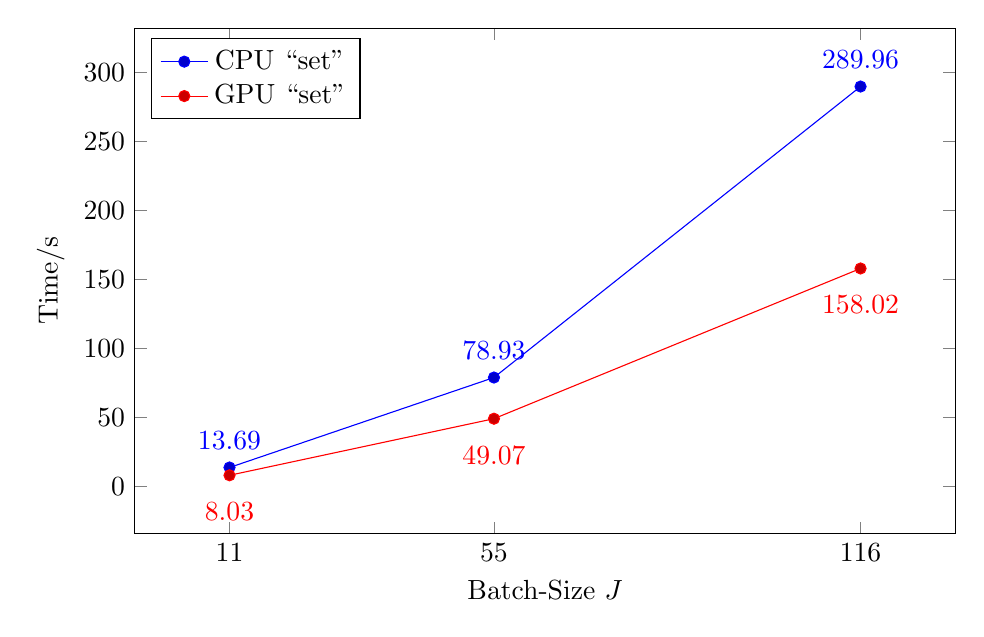
\begin{tikzpicture}
                \begin{axis}[
                    width=12cm,
                    height=8cm,
                    xtick=data,
                    xlabel={Batch-Size $J$},
                    ylabel={Time/s},
                    enlargelimits=0.15,
                    y tick label style={/pgf/number format/1000 sep=},
                    extra y tick style={grid=major, tick label style={xshift=-1cm}},
                    legend style={at={(0.02,.98)},
                        anchor=north west},
                    nodes near coords,
                    every node near coord/.append style={yshift=-0.7cm}
                ]
                \addplot+ [mark=*,,
                nodes near coords=\raisebox{0.8cm}{\pgfmathprintnumber\pgfplotspointmeta}
                ] coordinates {(11,13.69) (55,78.93) (116,289.96)};  % cpu
                \addplot+ [mark=*,] coordinates {(11,8.03) (55,49.07) (116,158.02)};  % gpu
                \legend{CPU ``set'',GPU ``set''}
                \end{axis}
            \end{tikzpicture}
            \caption{Time Taken by the Full Model: Unit increase in $J$ leads to 1.42 additional seconds with GPU ``set'', compared to 2.44 seconds with CPU ``set''.}
            \label{fig:Finding Rewards - Time Taken by the Full Model}
        \end{subfigure}\vspace*{1em}
        \begin{subfigure}{.49\textwidth}
            \centering
            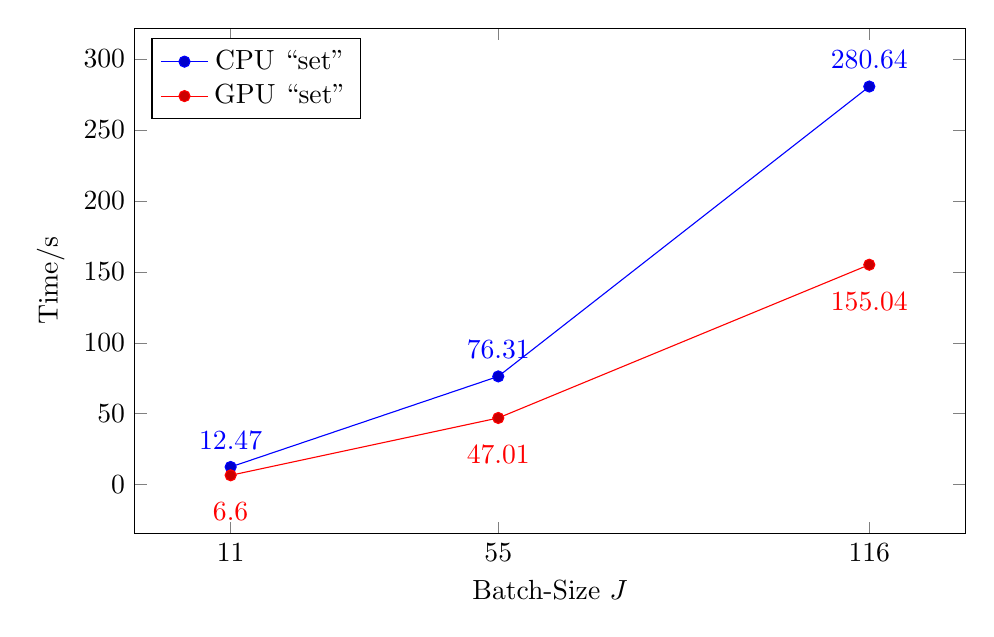
\begin{tikzpicture}
                \begin{axis}[
                    width=\textwidth,
                    height=8cm,
                    xtick=data,
                    enlargelimits=0.15,
                    xlabel={Batch-Size $J$},
                    ylabel={Time/s},
                    y tick label style={/pgf/number format/1000 sep=},
                    extra y tick style={grid=major, tick label style={xshift=-1cm}},
                    legend style={at={(0.02,.98)},
                        anchor=north west},
                    nodes near coords,
                    every node near coord/.append style={yshift=-0.7cm}
                ]
                \addplot+ [mark=*,
                nodes near coords=\raisebox{0.8cm}{\pgfmathprintnumber\pgfplotspointmeta}
                ] coordinates {(11,12.47) (55,76.31) (116,280.64)};  % cpu
                \addplot+ [mark=*,] coordinates {(11,6.60) (55,47.01) (116,155.04)};  % gpu
                \legend{CPU ``set'',GPU ``set''}
                \end{axis}
            \end{tikzpicture}
            \caption[Time taken by the LP]{Time taken by the LP: Unit increase in $J$ increases runtime by 1.41 seconds with GPU ``set''; 2.35 seconds with CPU ``set''}
            \label{fig:Finding Rewards - Time taken by the LP}
        \end{subfigure}\hspace*{1em}
        \begin{subfigure}{.49\textwidth}
            \centering
            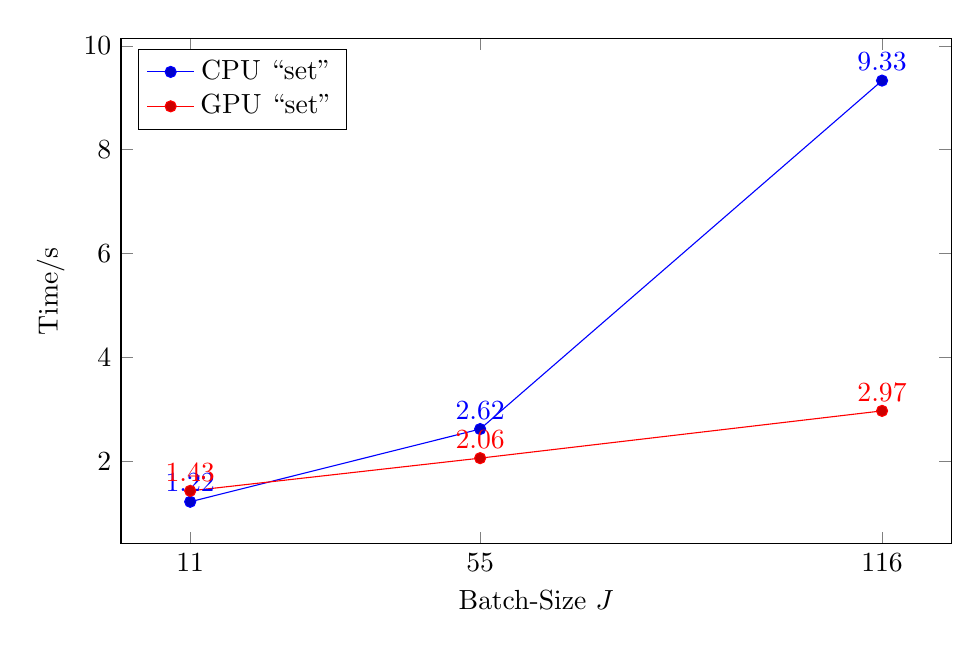
\begin{tikzpicture}
                \begin{axis}[
                    width=\textwidth,
                    height=8cm,
                    xtick=data,
                    xlabel={Batch-Size $J$},
                    ylabel={Time/s},
                    y tick label style={/pgf/number format/1000 sep=},
                    extra y tick style={grid=major, tick label style={xshift=-1cm}},
                    legend style={at={(0.02,.98)},
                        anchor=north west},
                    nodes near coords,
                ]
                \addplot+ [mark=*,] coordinates {(11,1.22) (55,2.62) (116,9.33)};  % cpu
                \addplot+ [mark=*,] coordinates {(11,1.43) (55,2.06) (116,2.97)};  % gpu
                \legend{CPU ``set'',GPU ``set''}
                \end{axis}
            \end{tikzpicture}
            \caption[Time taken by the Neural Network]{Time taken by the Neural Network: Unit increase in $J$ increases runtime by 0.0079 seconds with GPU ``set''; 0.0981 seconds with CPU ``set''}
            \label{fig:Finding Rewards - Time taken by the Neural Network}
        \end{subfigure}
        \vspace*{1em}
        \caption[Finding Rewards - Execution Times of Different Batch-Sizes $J$ with GPU and CPU ``set'' Separately]{Finding Rewards - Execution Times of Different Batch-Sizes $J$ with GPU and CPU ``set'' Separately: Scaling is strongly hampered by the LP solver. With GPU ``set'', while each unit increase in $J$ results in 0.0079 additional seconds for the Neural Network, it takes 1.41 seconds more for the LP.}
        \label{fig:Finding Rewards - Execution Times of Different Batch-Sizes J with GPU and CPU ``set'' Separately}
    \end{figure}

    Furthermore, although we expected SciPy's Optimize Module \cite{SCPOptimizeDocs} to run on the CPU (Section \ref{sec:Pricing Problem-Testing GPU Speedup on the Random Dataset}), the LP problem ran faster when the GPU was ``set''. We did not anticipate this behavior, and we couldn't pick out a reason for the Optimize Module supposedly doing operations differently. Since our GPU ``set'' and CPU ``set'' configurations were only enforceable on user-created functions and datasets, we do not know why the LP solver delivered different speeds while solving the same problem. If it used the CPU or the GPU, it should have done so in both cases and the runtime would have been equal. While there could be differences in implementation, we cannot affirm or deny any reason behind this quirky behavior. Figure \ref{fig:Finding Rewards - Time taken by the LP} shows the unexpected speedup of $\frac{2.35}{1.41} \approx 1.66$x delivered by SciPy Optimize Module's LP solver.
    
    \section{Conclusion} \label{sec:Conclusion}
    Our models for the Identification and the Pricing Problem outperformed previously studied ones and other baseline comparisons. For the Identification Problem, the average loss value was 12\% lower than the previous 2-layered model, and 35\% better than the 4-layered model, giving us better results than any other model. While we did not test deeper networks, we believe that using more hidden layers will only aggravate overfitting and won't provide better results - as is the case with the 4-layered network. The Pricing Problem's model also delivered better results than other baseline comparisons for reward distribution, though the difference was not drastically large.
    
    On the other hand, we can definitively conclude that these models ran faster on the GPU than the CPU, mainly because they were based on tensors and matrices. With an approximate speedup of 6.25 for unit increase in batch-size $T$ for the Identification Problem, we can scale to large datasets more efficiently on the GPU than the CPU. Although the Pricing Problem's model only delivered a speedup of ----- (with the LP problem heavily impacting the runtime), the 2-layered network for finding rewards gave a speedup of -----. This shows that neural network are inherently quick to optimize on a GPU. One can further use a GPU-accelerated LP solver or model the LP in the network itself (if possible) to get faster results.
    
    Figure \ref{fig:Plot for 3-layered Model} shows how the choice of Adam's algorithm \cite{Adam} for \textsc{Gradient-Descent}($\cdot$) helps the model to learn quickly. However, we also witness long periods of saturation after few epochs. This was the case for several other algorithms (SGD \cite{SGD} and Adagrad \cite{Adagrad}), but with different paces of learning. Since the organizers would want to further optimize the set of weights even, research could be done on avoiding the long, unchanging saturation phase. This may involve using other techniques for \textsc{Gradient-Descent}($\cdot$) (Algorithm \ref{alg:Algorithm for the Identification Problem}) and/or altering the loss function $Z_P(\matr{w_1}, \matr{w_2})$ (Equation \ref{eq:iden_problem}).
    
    One may also notice compelling arguments reflected by the results. Although these models are an \textit{upgrade} to the previous models, they deliver exciting inferences:
    \begin{itemize}
        \item One interesting observation in Table \ref{tab:Loss Values Calculated from Different Sets of Rewards} is that the Loss Value from the Proportional Distribution (0.161\%) and Random Initialization (0.160\%) are very close, highlighting that the set of weights obtained from the Identification Problem are dependent on other factors ($\matr{f}, \matr{D}$) as well and not just rewards. In other words, incentivizing under-sampled locations more is as good as random distribution of rewards - as agents don't get more heavily influenced by rewards than any other factor to visit locations.\\
        Moreover, by looking at the model's generated rewards, one can infer that the model chooses to place large rewards in 
    \end{itemize}
    
    
    \blindtext
    \bibliographystyle{IEEEtran}
    \bibliography{IEEEabrv,avicaching}
    
    \cleardoublepage
    \begin{appendices}
    \section{Implementation} \label{sec:Implementation}
    The code can be found here[]. \\
    Both the Identification and the Pricing Problem were programmed in Python 2.7 using NumPy 1.12.1, SciPy 0.19.1 and PyTorch 0.1.12 modules [web cites] \cite{SCPOptimizeDocs}\cite{NPDocs}. [Results from Python plotted in Matplotlib 2.0.2] With some code optimizations, the input dataset $\matr{F}$ was built using NumPy's \texttt{ndarray} and PyTorch's \texttt{tensor} functions. Since PyTorch offers NumPy-like code base but with dedicated neural network functions and submodules, PyTorch's \texttt{relu} and \texttt{softmax} functions were used along with other matrix operations.\\
    
    \subsection{Specific Implementation Details for the Pricing Problem}
    Among all the code optimizations in both models, some in that for the Pricing Problem are worth discussing, as they drastically differ from Algorithm \ref{alg:Solving the Pricing Problem} or are intricate. Most optimizations relevant to the Identification Problem are trivial and relate directly to those for the Pricing Problem. Therefore, only those in the Pricing Problem model are discussed.
    
    \subsubsection{Building the Dataset $\matr{F}$}
    Notice that we build the dataset $\matr{F}$ and batch-multiply it with $\matr{w_1}$ on each iteration/epoch (lines 2-3 of Algorithm \ref{alg:Solving the Pricing Problem}). Doing these steps are repetitive as most elements of $\matr{F}$, distances $\matr{D}$ and environmental feature vector $\vect{f}$, do not change unlike rewards $\vect{r}$. Moreover since $\matr{w_1}$ is fixed, Algorithm \ref{alg:Solving the Pricing Problem} would repetitively multiply the $\vect{f}$ and $\matr{D}$ components of $\matr{F}$ with $\matr{w_1}$. To avoid these unnecessary computations, we preprocessed most of $\matr{F}$ by batch-multiplying with $\matr{w_1}$ and only multiplied $\vect{r}$ with the corresponding elements of $\matr{w_1}$. Figure \ref{fig:Splitting and Batch Multiplying F and w1} describes the process graphically.\\
    \begin{figure}[!htbp]
        \centering
        \includegraphics[width=\linewidth]{split_and_batch_multiply}
        \caption{Splitting and Batch Multiplying $\matr{F}$ and $\matr{w_1}$}
        \label{fig:Splitting and Batch Multiplying F and w1}
    \end{figure}    
    Although this preprocessing might seem applicable for the model in Identification Problem too, it does not apply fully. Since the weights $\matr{w_1}$ are updated on each iteration/epoch, we cannot multiply them with parts of $\matr{F}$ beforehand (Algorithm \ref{alg:Algorithm for the Identification Problem}). However, we can combine $\matr{D}$ and $\vect{f}$ in the preprocessing stage and simply append $\vect{r}[t]$ on each iteration, saving computation time.
    
    \subsubsection{Modeling the Linear Programming Problem in the Standard Format}
    The \texttt{scipy.optimize} module's \texttt{linprog} function requires that the arguments are in standard LP format. As discussed in \cref{sec:Calculating Rewards}, Equation \ref{eq:lp_code_constrain_rewards} resembles the standard format more closely than \ref{eq:lp_math_constrain_rewards}, but it may not be clear how so.\\
    
    Considering $\vect{u}$ and $\vect{r'}$ as variables $\vect{x}$, Equation \ref{eq:lp_code_constrain_rewards} translates into Equation \ref{eq:lp_matrix_rewards} ($J$ is the number of locations).
    \begin{equation} \label{eq:lp_matrix_rewards}
    \begin{aligned}
    & \text{minimize}
    & & \begin{bmatrix}
    \vect{0_J}\\
    \vect{1_J}\\
    \end{bmatrix}^T
    \begin{bmatrix}
    \vect{r'}\\
    \vect{u}
    \end{bmatrix}\\ \\
    & \text{subject to}
    & & \begin{bmatrix}
    I_J & -I_J\\
    -I_J & -I_J\\
    \vect{1}^T_J & \vect{0}^T_J\\
    \end{bmatrix}
    \begin{bmatrix}
    \vect{r'}\\
    \vect{u}\\
    \end{bmatrix} \leq
    \begin{bmatrix}
    \vect{r}\\
    -\vect{r}\\
    \mathcal{R}\\
    \end{bmatrix}\\
    &&& r'_i, u_i \geq 0
    \end{aligned}
    \end{equation}
    
    \section{Strange GPU Speedup in LP Computation} \label{sec:Strange GPU Speedup in LP Computation}
    Even though we intentionally transferred the rewards vector to and constrained it using \texttt{scipy.optimize} module's \texttt{linprog} function on the CPU, we obtained an unexpected GPU speedup in the runtimes (see \cref{sec:PriProbRes - GPU} and Figure \ref{fig:Finding Rewards - Time taken by the LP}). Confounded by this weird behavior, we wanted to pinpoint the reasons because SciPy's function could not have differentiated between the configurations and delivered different results. However, since this was not our research's prime motive, we did not take a strong quantitative approach in determining the cause(s). There could have been many reasons for this bizarre behavior, including but not limited to:
    \begin{enumerate}
        \item SciPy's Optimize Module differentiating between configurations. This can be ruled out because the module could not have known the configuration during which it was called. This is because the configuration settings were applicable only on user-programmed operations, and needed to be explicitly stated - as mandated by PyTorch \cite{PTDocs}. SciPy's Optimize Module identifying the configurations is just supernatural.
        \item CPU ``set'' using exploiting more main memory than GPU ``set''. We suspected that since CPU ``set'' configuration's operations were executed solely on the CPU, the residing datasets could have used more main memory than when GPU ``set'' was running. This could have hampered the performance of LP with CPU ``set''. Unlike the 1\textsuperscript{st} possibility, this would have meant that CPU ``set'' was slowing down the LP, and not that GPU ``set'' was speeding up the LP.
    \end{enumerate}

    The 2\textsuperscript{nd} hypothesis/possibility seemed more promising than the others, and we built some programs to test its various aspects, which are elaborated in next sections.
    
    \subsection{Main Memory Usage by Both Configurations}
    As the initial approach, we logged details of main memory usage when the models were running. Contrary to our expectations (again), the GPU ``set'' was utilizing more main memory than CPU ``set'' was. Precisely, when running the Pricing Problem's model with $T = 173, J = 116$ without GUI and logging at 0.2 second intervals until the model completed, the GPU ``set'' was using 9.0 - 9.1 \% of the main memory, whereas CPU ``set'' was using only 0.9 \% memory. During the tests, only 1 CPU core was utilized for GPU ``set'', whereas 6-8 cores were being used for CPU ``set''. Clearly, main memory usage wouldn't have been the reason for the strange GPU speedup in LP runtime as LP's GPU ``set'' runtime would have been lower if the relation with main memory usage was true. However, there could be a relation between CPU usage and LP runtime.
    
    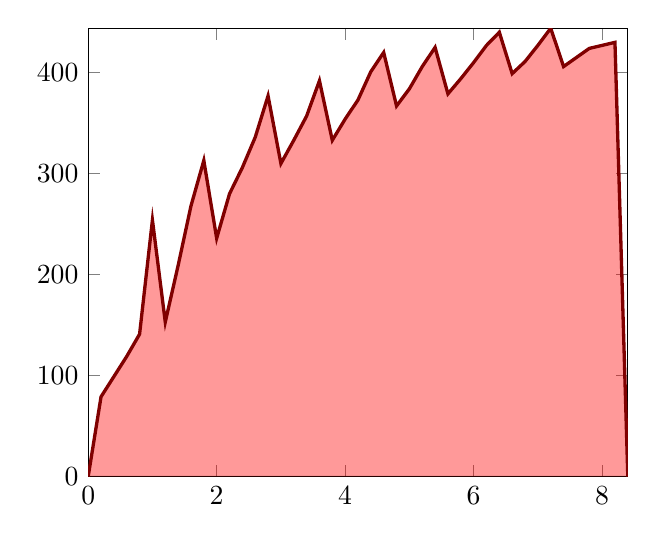
\begin{tikzpicture}
    \begin{axis}[
    domain=0:10,
    enlargelimits=false,
    ]
    %
    \addplot[fill=red, opacity=.4, domain=0:10] coordinates {
        (0.0, 0)
        (0.2, 79.0)
        (0.4, 99.0)
        (0.6, 119)
        (0.8, 141)
        (1.0, 254)
        (1.2, 153)
        (1.4, 209)
        (1.6, 268)
        (1.8, 313)
        (2.0, 236)
        (2.2, 280)
        (2.4, 306)
        (2.6, 336)
        (2.8, 377)
        (3.0, 310)
        (3.2, 333)
        (3.4, 357)
        (3.6, 392)
        (3.8, 333)
        (4.0, 354)
        (4.2, 373)
        (4.4, 401)
        (4.6, 420)
        (4.8, 367)
        (5.0, 384)
        (5.2, 406)
        (5.4, 425)
        (5.6, 379)
        (5.8, 394)
        (6.0, 410)
        (6.2, 427)
        (6.4, 440)
        (6.6, 399)
        (6.8, 411)
        (7.0, 427)
        (7.2, 444)
        (7.4, 406)
        (7.6, 415)
        (7.8, 424)
        (8.0, 427)
        (8.2, 430)
        (8.4, 0)
    }\closedcycle;
    
    \addplot [very thick, red!50!black] coordinates {
        (0.0, 0)
        (0.2, 79.0)
        (0.4, 99.0)
        (0.6, 119)
        (0.8, 141)
        (1.0, 254)
        (1.2, 153)
        (1.4, 209)
        (1.6, 268)
        (1.8, 313)
        (2.0, 236)
        (2.2, 280)
        (2.4, 306)
        (2.6, 336)
        (2.8, 377)
        (3.0, 310)
        (3.2, 333)
        (3.4, 357)
        (3.6, 392)
        (3.8, 333)
        (4.0, 354)
        (4.2, 373)
        (4.4, 401)
        (4.6, 420)
        (4.8, 367)
        (5.0, 384)
        (5.2, 406)
        (5.4, 425)
        (5.6, 379)
        (5.8, 394)
        (6.0, 410)
        (6.2, 427)
        (6.4, 440)
        (6.6, 399)
        (6.8, 411)
        (7.0, 427)
        (7.2, 444)
        (7.4, 406)
        (7.6, 415)
        (7.8, 424)
        (8.0, 427)
        (8.2, 430)
        (8.4, 0)
    };
    \end{axis}
    \end{tikzpicture}
    
    \subsubsection{asdf}
\end{appendices}
\end{document}